% ============================================================================
% Scale-Adaptive Geospatial Foundation-Model Dynamics
% for Baseline Land-Surface Change Prediction
% ============================================================================
% Target journal: Remote Sensing of Environment
% (Elsevier)
% ============================================================================
\ifdefined\pdfminorversion\pdfminorversion=5\fi
\ifdefined\pdfobjcompresslevel\pdfobjcompresslevel=0\fi
\documentclass{article}

\usepackage{amsmath,amssymb}
\usepackage{booktabs}
\usepackage{array}
\usepackage{graphicx}
\usepackage{multirow}
\usepackage{caption}
\usepackage{subcaption}
\usepackage{hyperref}
\usepackage{color}
\urlstyle{tt}

% Define keywords env for compile-anywhere only when the class does not provide it.
\makeatletter
\@ifundefined{keywords}{%
  \newenvironment{keywords}{\par\noindent\textbf{Keywords:} }{\par}%
}{}
\makeatother
\usepackage{natbib}
\usepackage{tikz}
\usetikzlibrary{positioning,arrows.meta,shapes.geometric,fit,calc}
\graphicspath{{../}{../figures/}{./figures/}{./paper8/figures/}{./}}
\bibliographystyle{plainnat}
\newcolumntype{P}[1]{>{\raggedright\arraybackslash}p{#1}}

\begin{document}

\makeatletter
\@ifundefined{ANONYMIZE}{
  \title{Scale-Adaptive Geospatial Foundation-Model Dynamics\\for Baseline Land-Surface Change Prediction}
  \author{Ning Zhou$^{a}$\\[0.3em]
  {\small $^{a}$SuperMap Software Co., Ltd., Beijing, China}\\
  {\small Correspondence: Ning Zhou}}
}{
  \title{Scale-Adaptive Geospatial Foundation-Model Dynamics\\for Baseline Land-Surface Change Prediction}
  \author{Anonymous authors}
}
\makeatother

\date{}
\maketitle

\begin{abstract}
Predicting land-use and land-cover (LULC) change from satellite observations is central to environmental remote sensing, yet many approaches either operate on categorical maps or require large pixel-level generative models. We introduce \textit{Scale-Adaptive Geospatial Foundation-Model Dynamics} (SA-GeoFMD), a frozen-encoder workflow that treats remote-sensing foundation-model embeddings as a compact predictive state space for annual land-surface dynamics. SA-GeoFMD combines AlphaEarth Foundations embeddings, a lightweight \textit{LatentDynamicsNet} (459K parameters) for residual embedding transitions, and a scale-adaptive spatial-demand allocation module for categorical LULC evaluation. On valid cached AlphaEarth study-area grids, the embedding dynamics have a positive mean advantage over persistence of +0.0047 cosine similarity, with 7 of 10 areas improving and a 95\% area-level bootstrap confidence interval of $[-0.0028, +0.0130]$. Independent ESRI-label validation on 12 area--year pairs gives non-zero categorical change signal: mean change F1 is 0.335, compared with 0.269 for a spatially shuffled control, 0.166 for a label-only transition-prior baseline, and 0.000 for persistence. In controlled same-grid comparisons with the GeoSOS-FLUS console allocator, the scale-adaptive categorical output improves the aggregate means for all four reported metrics on both the 24-township benchmark (change F1 0.286 vs.\ 0.267; FoM 0.125 vs.\ 0.121; transition accuracy 0.285 vs.\ 0.282; allocation disagreement 0.058 vs.\ 0.059, lower is better) and four external validation regions (0.312 vs.\ 0.291; 0.123 vs.\ 0.119; 0.282 vs.\ 0.275; 0.063 vs.\ 0.066). Across five GeoSOS-FLUS random seeds, SA-GeoFMD retains 5/5 overall wins for each metric in both validation groups. However, full-map end-year accuracy remains below persistence in the independent ESRI-label test, and some individual regions still show metric-specific losses. SA-GeoFMD is therefore best interpreted as a low-cost baseline-trend change-signal and controlled allocation workflow, not yet as a general counterfactual scenario simulator or universal operational LULC forecaster.
\end{abstract}

\begin{keywords}
remote-sensing foundation model; scale-adaptive geospatial dynamics; GeoSOS-FLUS; land-cover change; embedding-space forecasting; AlphaEarth
\end{keywords}

% ============================================================================
\section{Introduction}
\label{sec:intro}
% ============================================================================

Predicting how land surfaces will change over time is a central problem in geographical information science, with direct applications in urban planning, agricultural policy, ecological conservation, and climate adaptation \citep{verburg2004lulc}. Traditional approaches---cellular automata--Markov chains (CA-Markov), CLUE-S, and logistic regression---operate on categorical land-use maps, relying on hand-calibrated transition probabilities and socioeconomic driving factors \citep{veldkamp2004clues}. While effective in constrained scenarios, these methods cannot capture the rich, continuous spectral--spatial--temporal information present in modern satellite observations.

Recent advances in deep learning have introduced more powerful alternatives. Convolutional--recurrent architectures (ConvLSTM) can learn spatiotemporal patterns from classified imagery sequences \citep{shi2015convlstm}. EarthPT \citep{smith2023earthpt}, a 700M-parameter autoregressive transformer, predicts pixel-level spectral reflectance forward in time. DiffusionSat \citep{khanna2023diffusionsat} uses conditional diffusion models to generate future satellite images. However, all of these operate in raw observation space (spectral bands or classified pixels), inheriting two fundamental limitations: (1) prediction in high-dimensional pixel space is computationally expensive and prone to hallucination artifacts; and (2) pixel-level prediction conflates semantically meaningful change with irrelevant noise (cloud shadows, atmospheric variation, sensor calibration drift).

In the broader AI community, the concept of a \textit{world model}---a learned internal simulator that predicts environment state transitions in a compressed latent space---has emerged as a powerful paradigm for planning and reasoning. Pioneered by \citet{ha2018world} and advanced through the Dreamer family \citep{hafner2023dreamerv3} and MuZero \citep{schrittwieser2020muzero}, world models separate perception (encoding observations into latent states) from dynamics (predicting latent state transitions), enabling efficient forward simulation without rendering full observations. LeCun's JEPA framework \citep{lecun2022jepa} formalizes this principle: predict in representation space, not pixel space.

Simultaneously, geospatial foundation models (GeoFMs) have made pre-trained, high-quality representations of the Earth's surface freely available. AlphaEarth Foundations \citep{brown2025alphaearth} produces 64-dimensional L2-normalized embedding vectors at 10\,m resolution for every land pixel on Earth, annually from 2017 to 2024, derived from multi-sensor inputs (Sentinel-1/2, Landsat, GEDI, ERA5) via a 480M+ parameter vision transformer. These embeddings have been shown to be physically interpretable \citep{rahman2026interpretable} and linearly decodable to land-cover classes with $>$83\% accuracy.

This paper bridges these two developments through \textit{Scale-Adaptive Geospatial Foundation-Model Dynamics} (SA-GeoFMD): a workflow that treats GeoFM embeddings as the state space of a geospatial world model and uses a scale-aware allocation layer when categorical LULC maps are required for comparison. Our key insight is that if a foundation model has already learned to compress satellite observations into semantically meaningful, temporally varying embeddings, then the dynamics of land-use change can be learned \textit{on top of} these frozen embeddings using a lightweight neural network---without retraining the foundation model and without ever generating pixel-level predictions during dynamics training. This corresponds to the JEPA architecture: the foundation model serves as the encoder; a small LatentDynamicsNet serves as the predictor.

This work examines a specific and under-tested use of geospatial foundation models: whether a frozen, globally available embedding field can behave as a state variable for learned land-surface dynamics. The closest prior works either train their own encoder end-to-end (MM-VSF, \citealt{mmvsf2024}), operate in spectral space with larger autoregressive models (EarthPT), or predict downstream variables rather than the embeddings themselves (PDFM+TimesFM, \citealt{google2024pdfm}).

Our contributions are:

\begin{enumerate}
\item We formulate satellite-based LULC dynamics prediction as residual learning in a frozen remote-sensing foundation-model embedding space, and evaluate when this representation improves over persistence.

\item We design the \textit{LatentDynamicsNet}, a 459K-parameter dilated convolutional network with L2 manifold preservation and terrain context inputs for annual embedding-space prediction.

\item We introduce multi-step unrolled training loss to reduce exposure bias during autoregressive rollout and report development diagnostics for key architectural choices.

\item We add a scale-adaptive spatial-demand allocation module that converts decoded dynamics into calibrated categorical LULC maps while preserving small-region and large-region demand behavior.

\item We provide area-level diagnostics across cached Chinese study areas, including persistence comparisons, bootstrap uncertainty, encoder replacement, and change-focused evaluation where sufficient local evidence is available.

\item We add a reproducible empirical evidence-chain audit, an independent categorical change-label validation protocol, and same-grid GeoSOS-FLUS comparisons on both the original 24-township benchmark and four external validation regions.

\item We test downstream planning utility as an application probe by training reinforcement-learning policies on engineered land-planning features and frozen GeoFM embeddings. A feature-dropout ablation across 45 trained models (3 configurations $\times$ 15 seeds) quantifies when the embedding channel is helpful and when it is insufficient.
\end{enumerate}

Beyond forecasting, we use a controlled planning task to probe whether the same representation can provide complementary information when task-specific features are partially unavailable. Section~\ref{sec:planning} shows that reinforcement learning policies trained on task-specific features and GeoFM embeddings retain 87\% of full-information slope improvement under moderate feature dropout ($p=0.3$). Complete feature removal ($p=1.0$) reduces retention to 13\%, showing that the embedding channel is useful as a supplement but insufficient as a standalone planning state.


% ============================================================================
\section{Related Work}
\label{sec:related}
% ============================================================================

\subsection{LULC change prediction}

LULC change prediction has evolved from statistical models to deep learning approaches. CA-Markov \citep{veldkamp2004clues} combines cellular automata neighborhood rules with Markov chain transition matrices. CLUE-S \citep{verburg2002clues} incorporates logistic regression with socioeconomic drivers. More recently, Themeda \citep{turnbull2025themeda} uses ConvLSTM with 33 years of data and auxiliary climate variables, achieving 93.4\% pixel-wise accuracy for FAO Level 3 classes. TAMMs \citep{guo2025tamms} unifies temporal change description with future satellite image generation via MLLM and diffusion models.

\subsection{Earth observation foundation models}

GeoFMs have rapidly advanced. Prithvi-EO-2.0 \citep{jakubik2024prithvi} provides multi-temporal embeddings for classification tasks. SatMAE \citep{cong2022satmae} uses masked autoencoders with temporal positional encoding. Clay and Presto offer alternative embedding approaches. AlphaEarth Foundations \citep{brown2025alphaearth} stands out by providing annually-resolved, globally-available, 64-dimensional embeddings at 10\,m resolution through Google Earth Engine, with demonstrated physical interpretability \citep{rahman2026interpretable, benavides2026whatonearth}.

\subsection{World models and JEPA}

World models originated in reinforcement learning: Ha \& Schmidhuber's ``World Models'' \citep{ha2018world} learn compressed environment dynamics for policy training. Dreamer V3 \citep{hafner2023dreamerv3} achieves human-level performance across diverse domains using Recurrent State-Space Models (RSSMs). LeCun's JEPA \citep{lecun2022jepa} formalizes the principle of predicting in representation space rather than pixel space. AnySat \citep{astruc2024anysat} applies JEPA to remote sensing but for spatial mask prediction, not temporal dynamics. RemoteBAGEL \citep{remotebagel2025} proposes spatial extrapolation (generating adjacent tiles) but not temporal forecasting.

\subsection{Closest prior work}

MM-VSF \citep{mmvsf2024} predicts future satellite embeddings from current ones but trains its own encoder end-to-end rather than using a frozen foundation model. EarthPT \citep{smith2023earthpt} performs autoregressive prediction on raw spectral reflectance with 700M parameters. PDFM+TimesFM \citep{google2024pdfm} uses geospatial embeddings with a forecasting model but predicts socioeconomic variables, not the embeddings themselves. Our work focuses on the less explored setting of learning autoregressive dynamics \textit{on top of frozen GeoFM embeddings}.

\subsection{World models for decision making}

World models have been used as simulators for policy learning since \citet{ha2018world} trained RL agents inside learned latent dynamics. Dreamer V3 \citep{hafner2023dreamerv3} achieves human-level performance across 150+ tasks by learning policies entirely within a Recurrent State-Space Model. MuZero \citep{schrittwieser2020muzero} combines learned dynamics with Monte Carlo tree search for board games and Atari. In robotics, TD-MPC2 \citep{hansen2024tdmpc2} learns world models for continuous control. Section~\ref{sec:planning} uses land-use planning as a bounded application probe rather than as a complete operational planning system.


% ============================================================================
\section{Study Areas and Data}
\label{sec:data}
% ============================================================================

\subsection{Study areas}

We select 17 study areas across China, covering four major land-type categories, with a strict four-way split to evaluate generalization (Table~\ref{tab:areas}). Each area spans approximately 0.1\textdegree$\times$0.1\textdegree\ ($\approx$10\,km$\times$10\,km) at 10\,m resolution.

\begin{table}[htbp]
\centering
\caption{Study areas by split and land-type category.}
\label{tab:areas}
\begin{tabular}{llll}
\toprule
Split & Area name & Category & Bbox (WGS84) \\
\midrule
\multirow{12}{*}{Train (12)} & Yangtze Delta & Urban & [121.2, 31.0, 121.3, 31.1] \\
 & Jing-Jin-Ji & Urban & [116.3, 39.8, 116.4, 39.9] \\
 & Chengdu Plain & Urban & [104.0, 30.6, 104.1, 30.7] \\
 & NE Plain & Agriculture & [126.5, 45.7, 126.6, 45.8] \\
 & N.~China Plain & Agriculture & [115.0, 36.5, 115.1, 36.6] \\
 & Jianghan Plain & Agriculture & [113.5, 30.3, 113.6, 30.4] \\
 & Hetao & Agriculture & [107.0, 40.7, 107.1, 40.8] \\
 & Yunnan Eco & Ecology & [100.2, 25.0, 100.3, 25.1] \\
 & Daxinganling & Forest & [124.0, 50.3, 124.1, 50.4] \\
 & Qinghai Edge & Plateau & [101.5, 36.5, 101.6, 36.6] \\
 & Guanzhong & Mixed & [108.9, 34.2, 109.0, 34.3] \\
 & Minnan Coast & Mixed & [118.0, 24.4, 118.1, 24.5] \\
\midrule
\multirow{2}{*}{Val (2)} & Pearl River & Urban & [113.2, 23.0, 113.3, 23.1] \\
 & Poyang Lake & Wetland & [116.0, 29.0, 116.1, 29.1] \\
\midrule
Test (1) & Wuyi Mountain & Forest & [117.6, 27.7, 117.7, 27.8] \\
\midrule
\multirow{2}{*}{OOD (2)} & Sanxia Reservoir & Mixed & [110.3, 30.8, 110.4, 30.9] \\
 & Lhasa Valley & Plateau & [91.1, 29.6, 91.2, 29.7] \\
\bottomrule
\end{tabular}
\end{table}

\subsection{Data sources}

\textbf{AlphaEarth Embeddings.} We use the AlphaEarth annual satellite embedding dataset on Google Earth Engine (GEE; \url{GOOGLE/SATELLITE_EMBEDDING/V1/ANNUAL}), which provides 64-dimensional L2-normalized embedding vectors at 10\,m resolution for each year from 2017 to 2024. For each study area and year, 500 random pixel locations are sampled using \texttt{ee.Image.sample()} with \texttt{seed=42} for reproducibility, yielding $500\times64$ embedding matrices. All raw data are cached locally as NumPy \texttt{.npy} files for offline reproducibility.

\textbf{LULC Labels.} Land-cover class labels for decoder training are obtained from the ESRI Global LULC 10\,m Time Series on GEE (\url{projects/sat-io/open-datasets/landcover/ESRI_Global-LULC_10m_TS}), providing 9 land-cover classes at matching spatial resolution.

\textbf{Terrain Context.} DEM elevation and slope are derived from SRTM 30\,m (\texttt{USGS/SRTMGL1\_003}) via GEE. Elevation is min-max normalized to $[0,1]$; slope is clipped and normalized by 45\textdegree.

\textbf{Cadastral parcel data for downstream planning.} For the downstream planning experiment (Section~\ref{sec:planning}), we additionally use the cadastral parcel dataset for Bishan County, Chongqing, comprising 101{,}657 parcels aggregated into approximately 2{,}600 management blocks across three townships. Per-block features (17 dimensions) are computed from DEM-derived slope statistics, land-use class distributions, and boundary geometry. GeoFM embeddings (64 dimensions) for each block are obtained by spatially averaging AlphaEarth pixel embeddings within block boundaries.


% ============================================================================
\section{Methodology}
\label{sec:method}
% ============================================================================

\subsection{Architecture overview}

SA-GeoFMD follows a two-layer representation-dynamics architecture with an additional categorical allocation layer used only for LULC map evaluation (Fig.~\ref{fig:architecture}):

\begin{itemize}
\item \textbf{Layer 1: Frozen encoder.} AlphaEarth Foundations (480M+ parameters) maps satellite observations to 64-dimensional unit vectors. This layer is never trained; we consume its outputs as pre-computed embeddings.
\item \textbf{Layer 2: Learned dynamics.} LatentDynamicsNet (459K parameters) predicts the next year's embedding given the current embedding, a scenario encoding, and optional terrain context.
\item \textbf{Evaluation layer: Scale-adaptive allocation.} When categorical LULC maps are needed for comparison with cellular-automata baselines, decoded dynamics are passed through a calibrated spatial-demand allocation gate that controls the number and placement of predicted change pixels.
\end{itemize}

This corresponds to the JEPA framework \citep{lecun2022jepa}: the encoder produces representations; the predictor operates in representation space. The decoder (a linear classifier) is used only for visualization, not during dynamics prediction.

\begin{figure}[htbp]
\centering
\resizebox{\textwidth}{!}{%
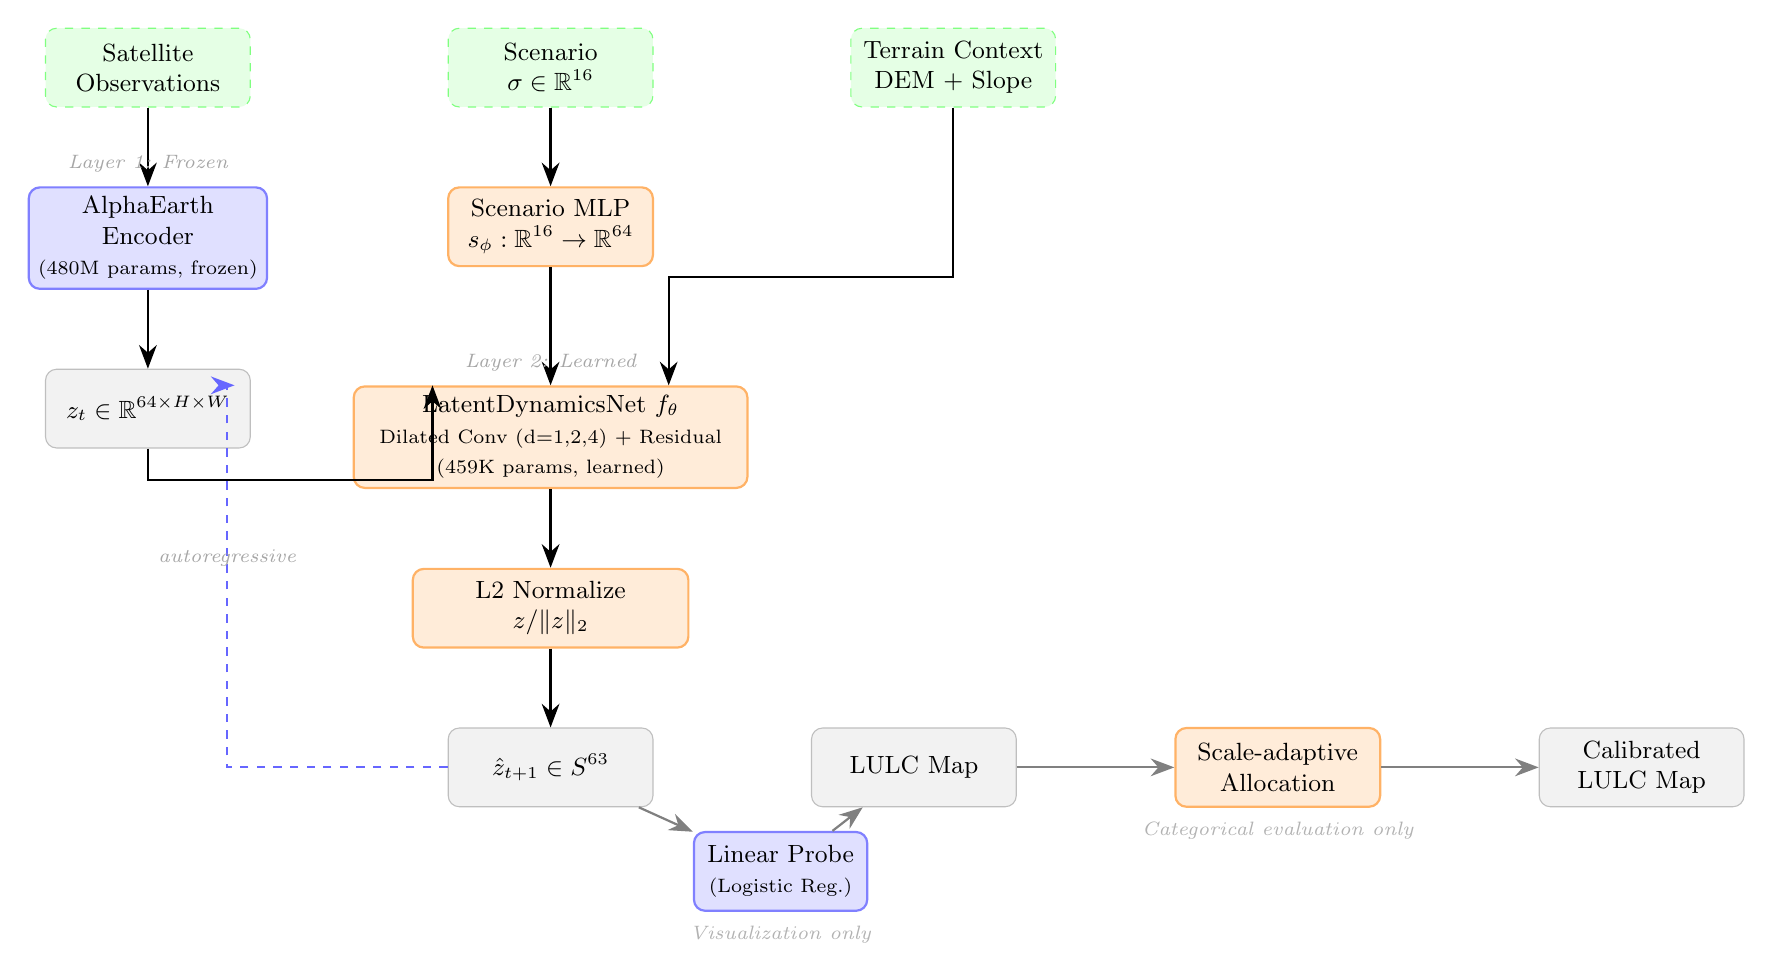
\begin{tikzpicture}[
    node distance=1.2cm and 1.8cm,
    box/.style={draw, rounded corners, minimum height=1.0cm, minimum width=2.6cm, align=center, font=\small},
    frozen/.style={box, fill=blue!12, draw=blue!50, thick},
    learned/.style={box, fill=orange!15, draw=orange!60, thick},
    input/.style={box, fill=green!10, draw=green!50, dashed},
    output/.style={box, fill=gray!10, draw=gray!50},
    arr/.style={-{Stealth[length=3mm]}, thick},
    label/.style={font=\scriptsize\itshape, text=gray!70},
]

% Row 1: Inputs
\node[input] (sat) {Satellite\\Observations};
\node[input, right=2.5cm of sat] (scenario) {Scenario\\$\sigma \in \mathbb{R}^{16}$};
\node[input, right=2.5cm of scenario] (terrain) {Terrain Context\\DEM + Slope};

% Row 2: Encoder + Scenario MLP
\node[frozen, below=1.0cm of sat] (encoder) {AlphaEarth\\Encoder\\{\scriptsize(480M params, frozen)}};
\node[learned, below=1.0cm of scenario] (smlp) {Scenario MLP\\$s_\phi: \mathbb{R}^{16} \to \mathbb{R}^{64}$};

% Row 3: Embedding
\node[output, below=1.0cm of encoder] (zt) {$z_t \in \mathbb{R}^{64 \times H \times W}$};

% Row 4: Dynamics
\node[learned, below=1.5cm of smlp, minimum width=5cm] (dynamics) {LatentDynamicsNet $f_\theta$\\{\scriptsize Dilated Conv (d=1,2,4) + Residual}\\{\scriptsize (459K params, learned)}};

% Row 5: Normalize
\node[learned, below=1.0cm of dynamics, minimum width=3.5cm] (norm) {L2 Normalize\\$z / \|z\|_2$};

% Row 6: Output + Decoder
\node[output, below=1.0cm of norm] (ztp1) {$\hat{z}_{t+1} \in S^{63}$};
\node[output, right=2.0cm of ztp1] (lulc) {LULC Map};
\node[learned, right=2.0cm of lulc, minimum width=2.6cm] (allocation) {Scale-adaptive\\Allocation};
\node[output, right=2.0cm of allocation] (calibrated) {Calibrated\\LULC Map};

% Decoder
\node[frozen, below right=0.3cm and 0.5cm of ztp1, minimum width=2.2cm] (decoder) {Linear Probe\\{\scriptsize(Logistic Reg.)}};

% Arrows: inputs to processing
\draw[arr] (sat) -- (encoder);
\draw[arr] (encoder) -- (zt);
\draw[arr] (scenario) -- (smlp);

% Concat arrows into dynamics
\draw[arr] (zt.south) -- ++(0,-0.4) -| ([xshift=-1.5cm]dynamics.north);
\draw[arr] (smlp.south) -- ([xshift=0cm]dynamics.north);
\draw[arr] (terrain.south) -- ++(0,-2.15) -| ([xshift=1.5cm]dynamics.north);

% Dynamics to normalize
\draw[arr] (dynamics) -- (norm);

% Normalize to output
\draw[arr] (norm) -- (ztp1);

% Autoregressive loop
\draw[arr, dashed, blue!60] (ztp1.west) -- ++(-2.8,0) |- ([xshift=-1.5cm]dynamics.north west) node[pos=0.25, above, label] {autoregressive};

% Decoder path
\draw[arr, gray] (ztp1) -- (decoder);
\draw[arr, gray] (decoder) -- (lulc);
\draw[arr, gray] (lulc) -- (allocation);
\draw[arr, gray] (allocation) -- (calibrated);

% Labels
\node[label, above=0.05cm of encoder] {Layer 1: Frozen};
\node[label, above=0.05cm of dynamics] {Layer 2: Learned};
\node[label, below=0.05cm of decoder, text=gray!60] {Visualization only};
\node[label, below=0.05cm of allocation, text=gray!60] {Categorical evaluation only};

\end{tikzpicture}
}
\caption{Architecture of the proposed SA-GeoFMD workflow following the JEPA paradigm. Layer~1 (blue, frozen) is the AlphaEarth foundation model encoder that maps satellite observations to 64-dimensional unit-vector embeddings. Layer~2 (orange, learned) is the LatentDynamicsNet that predicts residual state transitions in embedding space, with explicit L2 re-normalization after each step. The dashed blue arrow represents the autoregressive feedback loop during multi-step rollout. The linear probe decoder (gray) and scale-adaptive allocation layer are used for LULC visualization and categorical comparison, not during dynamics prediction. Scenario inputs are reserved by the architecture but only the baseline trajectory is trained and evaluated in this paper.}
\label{fig:architecture}
\end{figure}

\subsection{LatentDynamicsNet}
\label{sec:network}

The dynamics model predicts the residual change in embedding space:
\begin{equation}
\hat{z}_{t+1} = \text{normalize}\Big(z_t + f_\theta\big([z_t \,\|\, s_\phi(\sigma) \,\|\, c]\big)\Big)
\label{eq:dynamics}
\end{equation}
where $z_t \in \mathbb{R}^{64 \times H \times W}$ is the current embedding grid, $\sigma \in \mathbb{R}^{16}$ is the scenario encoding, $s_\phi: \mathbb{R}^{16} \to \mathbb{R}^{64}$ is a two-layer MLP that maps the scenario to embedding dimension and broadcasts spatially, $c \in \mathbb{R}^{2 \times H \times W}$ is the terrain context (DEM elevation + slope), and $\text{normalize}(\cdot)$ denotes L2 normalization along the channel dimension.

The dynamics function $f_\theta$ is a dilated convolutional network:
\begin{equation}
\begin{aligned}
f_\theta ={}& \text{Conv}_{1\times1}^{128 \to 64} \circ \text{GN-GELU}
\circ \text{DilConv}_{3\times3}^{d=4} \circ \text{GN-GELU} \\
& \circ \text{DilConv}_{3\times3}^{d=2} \circ \text{GN-GELU}
\circ \text{DilConv}_{3\times3}^{d=1}.
\end{aligned}
\end{equation}
where DilConv denotes dilated convolution with the specified dilation rate, and GN-GELU denotes GroupNorm (8 groups) followed by GELU activation. The input to the first layer has $64 + 64 + 2 = 130$ channels (embedding + scenario + terrain context). Dilation rates of 1, 2, 4 yield a theoretical receptive field of 17$\times$17 pixels (170\,m at 10\,m resolution), allowing local context to include features such as road construction edges or urban expansion fronts.

\textbf{Design rationale.} (1) \textit{Residual connection}: inter-annual embedding change is small (cosine similarity $\approx$0.96); learning the residual $\Delta z = f_\theta(\cdot)$ rather than the absolute $z_{t+1}$ avoids the identity-mapping collapse. (2) \textit{GroupNorm}: with only 60 training samples, BatchNorm statistics are unreliable; GroupNorm is batch-size invariant. (3) \textit{L2 normalization}: AlphaEarth embeddings lie on the 64-dimensional unit hypersphere; without explicit re-projection after residual addition, the embeddings drift off-manifold, causing downstream decoder failure (Section~\ref{sec:manifold}).

\subsection{Baseline dynamics and scenario placeholder}

The architecture includes a scenario encoding vector $\sigma \in \mathbb{R}^{16}$ so that future versions can condition dynamics on policy or environmental drivers. In the experiments reported here, however, all observed historical transitions are treated as the baseline trajectory. The scenario input is therefore fixed to the baseline index during training and evaluation.

\textbf{Scope of the present model.} The current model should be understood as a \textit{baseline-trend predictor}. We do not report counterfactual policy-scenario results, because non-baseline scenario weights have not received direct supervision. Activating scenario-conditioned counterfactual simulation would require scenario-labelled historical interventions, policy-specific constraints, or another source of supervised counterfactual signal.

\begin{table}[htbp]
\centering
\caption{Scenario indices reserved by the architecture. Only the baseline input is trained and evaluated in this study.}
\label{tab:scenarios}
\small
\begin{tabular}{clp{0.55\textwidth}}
\toprule
ID & Name & Description \\
\midrule
0 & Urban sprawl & Reserved; not evaluated here \\
1 & Ecological restoration & Reserved; not evaluated here \\
2 & Agricultural intensification & Reserved; not evaluated here \\
3 & Climate adaptation & Reserved; not evaluated here \\
4 & Baseline & Historical trend continuation; trained and evaluated \\
\bottomrule
\end{tabular}
\end{table}

\subsection{Manifold preservation via L2 normalization}
\label{sec:manifold}

AlphaEarth embeddings are L2-normalized unit vectors. The residual operation $z + \Delta z$ does not preserve unit norm. Over $k$ autoregressive steps, the embedding norm diverges as $\|z_k\| \neq 1$, causing the downstream linear decoder (trained on unit vectors) to encounter out-of-distribution inputs.

We enforce manifold preservation by re-normalizing after each step:
\begin{equation}
z_{t+1} = \frac{z_t + f_\theta(z_t, s, c)}{\|z_t + f_\theta(z_t, s, c)\|_2}
\end{equation}

We verify empirically that after 20 autoregressive steps, all pixel vectors maintain $\|z\|_2 = 1.0$ with error $<10^{-5}$.

\subsection{Multi-step unrolled training}
\label{sec:multistep}

Standard single-step training (teacher forcing) creates exposure bias: the model is trained with ground-truth inputs but at inference must consume its own predictions. To mitigate this, we unroll the autoregressive loop for $K=3$ steps during training and compute a weighted sum of losses:
\begin{equation}
\mathcal{L} = \sum_{k=1}^{K} \frac{1}{2^{k-1}} \|\hat{z}_{t+k} - z_{t+k}\|_2^2
\end{equation}
where $\hat{z}_{t+k}$ is the $k$-step predicted embedding (each step using the previous prediction as input) and $z_{t+k}$ is the ground truth. The exponentially decaying weights prioritize short-term accuracy while still encouraging long-horizon consistency.

\subsection{LULC decoder}

Predicted embeddings can be decoded to LULC classes for visualization using a linear probe (scikit-learn LogisticRegression, max\_iter=1000). The probe is trained on 2020 AlphaEarth embeddings paired with ESRI Global LULC labels. A traceable 5-fold cross-validation run over six ESRI class codes gives 76.99\% overall accuracy over 5,119 samples. This decoder is not used for dynamics training, and embedding-space cosine similarity remains the primary evaluation metric.

\subsection{Scale-adaptive spatial-demand allocation}
\label{sec:scale_adaptive_allocation}

Decoded LULC maps from embedding dynamics can over-predict change area, especially when the candidate region is much larger than the calibration townships. To make categorical comparisons more conservative and reproducible, SA-GeoFMD applies a spatial-demand allocation gate after decoding. This gate is not used during embedding training. It only converts the decoded baseline-trend prediction into a calibrated categorical map for metrics such as change F1, figure of merit (FoM), transition accuracy, and allocation disagreement.

For each target area, candidate change pixels are those where the decoded prediction differs from the start-year reference map. Let $p_c$ be the candidate change fraction and let $p^\ast$ be the calibrated target change fraction. We estimate a ratio model from calibration areas:
\begin{equation}
p^\ast = \mathrm{clip}\left(p_c \, r_q \, m(A),\, p_{\min},\, p_{\max}\right),
\end{equation}
where $r_q$ is the $q=0.25$ quantile of observed-to-candidate change ratios in the calibration set, $p_{\min}=0.05$, $p_{\max}=0.25$, and $m(A)$ is a scale-dependent multiplier. The final audited configuration uses $m(A)=1.5$ for regions with fewer than 50{,}000 valid pixels and $m(A)=3.0$ otherwise. This rule preserves the audited small-region behavior observed on the 24-township benchmark while allowing larger external validation regions to keep enough candidate changes to avoid systematic under-prediction.

The allocation gate then ranks candidate change pixels using the change score, multi-scale class-aligned neighborhood support, and transition reliability estimated from held-out calibration labels. The final score adds target-neighborhood support with weight 1.5, subtracts source-neighborhood support with weight 0.65, and adds transition-reliability support with weight 0.6 across neighborhood windows of 3, 5, and 9 pixels. The highest-ranked candidates are retained until the target change budget is reached; all other candidate pixels revert to the start-year class. The manifest for each run records the valid-pixel count, selected multiplier, target change fraction, and retained change pixels, making the allocation step auditable.

\subsection{Inference procedure}

Given a bounding box and prediction horizon $N$:
\begin{enumerate}
\item Extract year-$t$ AlphaEarth embeddings from GEE.
\item Optionally extract DEM/slope terrain context.
\item Encode the baseline trajectory as a 16-dimensional vector.
\item Autoregressive loop: for $k = 1, \ldots, N$, compute $z_{t+k}$ via Eq.~\ref{eq:dynamics} with L2 normalization.
\item Optionally decode $z_{t+k}$ to LULC classes for visualization; quantitative dynamics evaluation remains in embedding space.
\end{enumerate}


% ============================================================================
\section{Experiments}
\label{sec:experiments}
% ============================================================================

\subsection{Experimental setup}

\textbf{Data splits.} The development workflow used 12 training areas, 2 validation areas, 1 test area, and 2 out-of-distribution areas. Gridded cached embeddings support the convolutional dynamics model, while point-sampled embeddings are used only for lightweight feasibility and diagnostic checks. In the revised data-traceable summary, area-level statistics are reported only for cached grids with valid non-placeholder metrics.

\textbf{Training.} Adam optimizer ($\text{lr} = 10^{-3}$), 100 epochs, 3-step unrolled loss with decaying weights $[1.0, 0.5, 0.25]$. Training completes in $\approx$80\,s on CPU (Intel i7-12700). No GPU required.

\textbf{Metrics.} (1) Cosine similarity between predicted and ground-truth embeddings (primary metric). (2) Mean squared error (MSE). (3) L2 distance. All metrics are computed per-pixel and averaged.

\subsection{Baseline methods}

\begin{itemize}
\item \textbf{Persistence:} $\hat{z}_{t+1} = z_t$ (``next year equals this year'')---the standard naive baseline in time-series forecasting.
\item \textbf{Linear extrapolation:} $\hat{z}_{t+1} = 2z_t - z_{t-1}$ (linear trend continuation).
\item \textbf{Label-only transition prior:} for categorical validation only, we estimate empirical start-class to end-class transition frequencies from other available ESRI label pairs with the same grid shape and apply those frequencies to the target start-year map. This baseline uses no AlphaEarth embeddings and no LatentDynamicsNet prediction, so it tests whether apparent change detection is explained only by coarse class-transition frequencies.
\end{itemize}

\subsection{Change-pixel evaluation protocol}

Global cosine similarity is dominated by pixels with weak annual embedding displacement. To diagnose whether the model captures localized dynamics rather than only predicting stasis, we stratify evaluation:
\begin{itemize}
\item \textbf{Changed pixels:} top 20\% by L2 distance between $z_t$ and $z_{t+1}$ (embedding-displacement proxy).
\item \textbf{Stable pixels:} bottom 20\% by the same distance.
\end{itemize}
This diagnostic tests whether the model captures representation dynamics or merely predicts stasis; it is not a substitute for independent labelled land-cover change validation.

\subsection{Independent categorical change-validation protocol}
\label{sec:independent_change_protocol}

To convert the embedding-displacement diagnostic into a formal land-cover transition test, we implemented a separate validation protocol that operates on annual categorical LULC maps. The protocol requires three co-registered arrays for each area--year pair: the reference start-year map $y_t$, the reference end-year map $y_{t+1}$, and the decoded model prediction $\hat{y}_{t+1}$. Reference labels and predicted maps are stored under \path{data/independent_change_labels/labels} and \path{data/independent_change_labels/predicted}, respectively, using area and year identifiers in the filenames. A persistence baseline is computed internally as $\hat{y}_{t+1}=y_t$.

The validation script reports binary change precision, recall, and F1; end-year categorical accuracy; accuracy on truly changed pixels; exact transition-match accuracy on changed pixels; and class-area bias measured as the mean absolute difference between predicted and reference class fractions. We include two controls beyond persistence. First, a spatially shuffled model negative control randomly permutes the predicted end-year map with a fixed seed, preserving the predicted class histogram while destroying spatial correspondence. This control tests whether the decoded dynamics carry spatially localized transition information rather than only predicting plausible class proportions. Second, a label-only transition prior estimates empirical categorical transition frequencies from other available ESRI label pairs and applies those frequencies to the target start-year map without using embeddings or model predictions. This tests whether the model's change signal is stronger than a simple categorical transition-frequency prior. The script writes per-area CSV rows and transition-count tables. The current repository audit contains 12 completed independent area--year pairs across Banzhucun, Bishan, Heping, Poyang Lake, and Wuyi Mountain, with no skipped label--prediction pairs in the current cache.

\subsection{Same-grid GeoSOS-FLUS comparison protocol}
\label{sec:geosos_flus_protocol}

We further compare SA-GeoFMD with the GeoSOS-FLUS console implementation under a controlled same-grid protocol. The comparison isolates the final categorical allocation problem rather than attempting a full native GeoSOS-FLUS deployment. Both methods operate on the same start-year map, label grid, and target evaluation mask, and GeoSOS-FLUS is configured from prediction-side suitability and demand information rather than from target end-year truth. This design avoids giving the cellular-automata baseline access to reference change while keeping the evaluation grid identical. It should not be read as a production GeoSOS-FLUS experiment with locally calibrated ANN drivers and full socioeconomic or biophysical covariates.

Two validation groups are used. The first is the original 24-township same-grid benchmark, which contains township-scale samples with 3,176--37,126 valid pixels. The second contains four larger external regions (Dongguan, Kunshan, Anxin, and Caidian) with 50,634--421,812 valid pixels. The scale-adaptive allocation rule described in Section~\ref{sec:scale_adaptive_allocation} therefore uses the small-region multiplier for all 24 township samples and the large-region multiplier for all four external samples. For each group, we report mean change F1, FoM, transition accuracy on true changed pixels, and allocation disagreement. We also run five GeoSOS-FLUS random seeds (1001--1005) and summarize overall mean deltas relative to GeoSOS-FLUS.

\subsection{Empirical evidence chain and validation boundary}
\label{sec:evidence_chain}

To make the empirical workflow auditable, we summarize the evidence chain used in the revised manuscript and maintain the same classification in a machine-readable audit file generated by the revision audit script. The audit distinguishes results that directly support the main embedding-space claim from diagnostic probes that support bounded interpretation but not standalone operational claims. Table~\ref{tab:empirical_pipeline} is therefore part of the empirical design rather than a post hoc disclaimer.

\begin{table}[htbp]
\centering
\caption{Empirical evidence chain and validation boundary for the revised manuscript. ``Complete'' means that a traceable result file directly supports the stated manuscript claim. ``Diagnostic'' means that the result is used for interpretation or application probing only. ``Missing'' means that the stage is not used as completed evidence in this paper.}
\label{tab:empirical_pipeline}
\footnotesize
\setlength{\tabcolsep}{2pt}
\begin{tabular}{@{}P{0.20\textwidth}P{0.13\textwidth}P{0.35\textwidth}P{0.26\textwidth}@{}}
\toprule
Empirical stage & Status & Evidence in this manuscript & Boundary / next validation \\
\midrule
Area-level embedding dynamics & Complete & 10 valid cached AlphaEarth grids; mean model-minus-persistence advantage +0.0047; 7/10 areas positive. & Supports bounded baseline-trend prediction in embedding space. \\
Encoder replacement ablation & Complete & Prithvi-100M CLS branch on 17 areas; mean advantage $-2.4 \times 10^{-6}$. & Representation-state diagnostic, not a dense-token Prithvi benchmark. \\
Semantic decoder validation & Diagnostic & Logistic-regression decoder on 5,119 AlphaEarth--ESRI samples; overall accuracy 76.99\%, macro-F1 0.668. & Supports qualitative decoding, not transition-level validation. \\
Planning feature dropout & Diagnostic & 45 trained policies; dropout 0.3 retains 86.8\% of full-feature slope improvement; embedding-only retains 12.9\%. & Application probe, not operational planning deployment. \\
Embedding-space transfer probe & Diagnostic & Banzhucun $\to$ Heping policy improves reward by +5.5 vs.\ random and +13.1 vs.\ greedy. & Weak zero-shot signal within one diagnostic reward system. \\
Independent change-label validation & Complete & 12 ESRI-label pairs; model change F1 0.335 vs.\ shuffled 0.269, transition prior 0.166, and persistence 0.000; changed-pixel accuracy 0.279. & Positive but region-dependent change signal; end-year categorical accuracy and class-area bias remain weaker than simple map-level baselines. \\
Same-grid GeoSOS-FLUS comparison & Complete & 24-township benchmark and four external regions; SA-GeoFMD improves all four aggregate mean metrics in both groups; five-seed overall wins are 5/5 for all four metrics in both groups. & Same-grid allocation benchmark using prediction-derived GeoSOS-FLUS demand/suitability, not a full native-driver FLUS deployment. \\
\bottomrule
\end{tabular}
\end{table}


% ============================================================================
\section{Results}
\label{sec:results}
% ============================================================================

\subsection{Phase 0: Embedding feasibility}

Before training any dynamics model, we verified three prerequisites on 3 areas $\times$ 7 years $\times$ 500 points:

\begin{table}[htbp]
\centering
\caption{Phase 0 feasibility validation results.}
\label{tab:phase0}
\begin{tabular}{lccc}
\toprule
Criterion & Threshold (pass/strong) & Result & Verdict \\
\midrule
Interannual cos.~sim. & $<$0.99 / $<$0.95 & 0.953 & PASS \\
Change/stable separation & $>$2$\times$ / $>$5$\times$ & 2.44$\times$ & PASS \\
Linear decode accuracy & $>$50\% / $>$70\% & 76.99\% & STRONG \\
\bottomrule
\end{tabular}
\end{table}

\subsection{Aggregate results}

\begin{table}[htbp]
\centering
\caption{Data-traceable area-level prediction quality from valid cached AlphaEarth grids (1-step, cosine similarity). Confidence intervals are non-parametric bootstrap intervals over area-level means.}
\label{tab:aggregate}
\begin{tabular}{lccc}
\toprule
Metric & $n$ areas & Mean & 95\% CI \\
\midrule
Persistence & 10 & 0.9757 & [0.9675, 0.9832] \\
LatentDynamicsNet & 10 & 0.9804 & [0.9757, 0.9852] \\
Model $-$ persistence & 10 & +0.0047 & [$-$0.0028, +0.0130] \\
\bottomrule
\end{tabular}
\end{table}

Across valid cached AlphaEarth grids, the model improved over persistence in 7 of 10 areas (two-sided sign-test $p=0.344$). The mean area-level advantage was positive (+0.0047 cosine similarity), but the bootstrap confidence interval crossed zero. We therefore interpret the result as evidence that frozen GeoFM embeddings can support useful baseline-trend dynamics in some regions, rather than as a universal improvement over persistence.

\subsection{Per-area results}

\begin{table}[htbp]
\centering
\caption{Per-area 1-step prediction quality for valid cached AlphaEarth grids.}
\label{tab:perarea}
\begin{tabular}{lccc}
\toprule
Area & Model & Persistence & Advantage \\
\midrule
Qinghai Edge & 0.9789 & 0.9489 & \textbf{+0.0300} \\
Jianghan Plain & 0.9862 & 0.9639 & \textbf{+0.0223} \\
Poyang Lake & 0.9855 & 0.9735 & \textbf{+0.0120} \\
Jing-Jin-Ji & 0.9751 & 0.9713 & +0.0039 \\
Minnan Coast & 0.9931 & 0.9908 & +0.0023 \\
Yangtze Delta & 0.9917 & 0.9910 & +0.0007 \\
Chengdu Plain & 0.9716 & 0.9708 & +0.0007 \\
Pearl River & 0.9786 & 0.9803 & $-$0.0017 \\
Bishan & 0.9719 & 0.9781 & $-$0.0062 \\
Daxinganling & 0.9714 & 0.9882 & $-$0.0168 \\
\bottomrule
\end{tabular}
\end{table}

The largest positive advantages occur in Qinghai Edge, Jianghan Plain, and Poyang Lake. Negative cases occur in Bishan, Daxinganling, and Pearl River, indicating that the learned residual dynamics can underperform persistence when inter-annual drift is weak or when the cached region differs from the model's strongest training domains.

Table~\ref{tab:category_diagnostic} groups the same area-level results by the study-area categories in Table~\ref{tab:areas}. The grouping is diagnostic because most categories contain only one or two valid cached areas. It nevertheless helps explain the region dependence: the four urban areas are close to neutral on average, while the strongest positive and negative results occur in single-area plateau/agriculture and forest cases, respectively.

\begin{table}[htbp]
\centering
\caption{Diagnostic grouping of AlphaEarth area-level advantage by study-area category. The table summarizes valid cached areas only and should not be interpreted as a formal biome-level statistical test.}
\label{tab:category_diagnostic}
\small
\begin{tabular}{lccc}
\toprule
Category & Valid areas & Mean advantage & Positive / negative \\
\midrule
Urban & 4 & +0.0009 & 3 / 1 \\
Agriculture & 1 & +0.0223 & 1 / 0 \\
Wetland & 1 & +0.0120 & 1 / 0 \\
Plateau & 1 & +0.0300 & 1 / 0 \\
Mixed & 2 & $-$0.0019 & 1 / 1 \\
Forest & 1 & $-$0.0168 & 0 / 1 \\
\bottomrule
\end{tabular}
\end{table}

\subsection{Change-pixel analysis}

\begin{table}[htbp]
\centering
\caption{Change-pixel diagnostic on the currently traceable cached region. Changed pixels are the top 20\% by embedding displacement.}
\label{tab:changepixel}
\begin{tabular}{lcccc}
\toprule
Area & Model & Persist. & Advantage & Source \\
\midrule
Bishan & 0.955710 & 0.955734 & $-2.35 \times 10^{-5}$ & cached grid \\
\bottomrule
\end{tabular}
\end{table}

The current change-pixel analysis should be read as a narrow diagnostic rather than an independent land-cover validation. Changed pixels are defined by high embedding displacement, not by manually interpreted land-cover transitions. In the traceable cached result, the changed-pixel advantage is effectively zero and slightly negative in Bishan. This does not support a general claim that the model is stronger on changed pixels. The independent validation in Section~\ref{sec:independent_change_validation} therefore provides the more relevant categorical transition test.

\subsection{Independent categorical change validation}
\label{sec:independent_change_validation}

We evaluated decoded model predictions against independently extracted ESRI Global LULC annual labels on 12 area--year pairs with matching cached prediction grids (Table~\ref{tab:independent_change_validation}). The evaluated set includes two Banzhucun three-year windows, seven annual Bishan windows, one Heping three-year window, and two held-out validation/test-area windows from Poyang Lake and Wuyi Mountain. Reference change rates range from 0.0\% in Wuyi Mountain 2020--2021 to 26.9\% in Banzhucun 2020--2023.

\begin{table}[htbp]
\centering
\caption{Independent categorical change validation against ESRI annual LULC labels. Change metrics treat a pixel as changed when the end-year class differs from the start-year class. The shuffled control randomly permutes the model-predicted end-year map, preserving predicted class frequencies while removing spatial correspondence. The transition-prior baseline uses empirical class-transition frequencies from other label pairs with the same grid shape and contains no embedding or model-prediction information. Persistence predicts the end-year map as identical to the start-year map.}
\label{tab:independent_change_validation}
\scriptsize
\setlength{\tabcolsep}{2pt}
\resizebox{\textwidth}{!}{%
\begin{tabular}{lcccccccc}
\toprule
Area--years & Chg. \% & Model F1 & Shuf. F1 & Prior F1 & Chg.-pix. acc. & Model end acc. & Prior end acc. & Pers. end acc. \\
\midrule
Banzhucun 2017--2020 & 22.1 & 0.371 & 0.335 & 0.226 & 0.303 & 0.535 & 0.667 & 0.779 \\
Banzhucun 2020--2023 & 26.9 & 0.482 & 0.417 & 0.297 & 0.292 & 0.558 & 0.656 & 0.731 \\
Bishan annual mean (7 pairs) & 14.5 & 0.344 & 0.254 & 0.177 & 0.342 & 0.641 & 0.749 & 0.855 \\
Heping 2017--2020 & 16.8 & 0.375 & 0.317 & 0.235 & 0.191 & 0.676 & 0.772 & 0.832 \\
Poyang Lake 2020--2021 & 17.4 & 0.385 & 0.389 & 0.000 & 0.163 & 0.743 & 0.826 & 0.826 \\
Wuyi Mountain 2020--2021 & 0.0 & 0.000 & 0.000 & 0.000 & 0.000 & 0.996 & 1.000 & 1.000 \\
\midrule
Mean (12 pairs) & 15.4 & 0.335 & 0.269 & 0.166 & 0.279 & 0.666 & 0.764 & 0.846 \\
\bottomrule
\end{tabular}
}
\end{table}

The independent validation changes the interpretation of the model. Because persistence predicts no categorical changes, its binary change F1 and changed-pixel transition accuracy are zero by construction; the model obtains a mean change F1 of 0.335 and a mean changed-pixel accuracy of 0.279. The spatially shuffled negative control reaches a lower mean change F1 of 0.269, and the label-only transition prior reaches 0.166. This indicates that part of the model's change signal is spatially localized and stronger than a simple categorical transition-frequency prior. However, this advantage is not uniform: in Poyang Lake the shuffled control is marginally higher than the model on binary change F1, and Wuyi Mountain contains no ESRI-labelled categorical change in 2020--2021. The model's overall end-year categorical accuracy remains lower than persistence (0.666 vs.\ 0.846) and lower than the transition prior (0.764), and its class-area bias is also larger than both map-level baselines. The evidence therefore supports a bounded claim: the latent dynamics can identify some changing pixels and transitions, but it is not yet a superior full-map categorical LULC forecaster.

\begin{figure}[htbp]
\centering
\includegraphics[width=\textwidth]{figures/fig_rse_revision_spatial_change_validation.pdf}
\caption{Spatial validation and failure-mode example for Banzhucun 2020--2023. Panels show the reference start-year map, reference end-year map, decoded model prediction, binary reference change, binary predicted change, and change-detection error classes. The model detects many true changed pixels (36,605 hits) but also produces substantial false alarms (55,763) and misses (22,983), illustrating why change F1 improves over controls while full-map categorical accuracy remains below persistence.}
\label{fig:spatial_change_validation}
\end{figure}

\subsection{Same-grid comparison with GeoSOS-FLUS}
\label{sec:geosos_flus_results}

The scale-adaptive allocation module changes the categorical evaluation picture relative to the raw decoded dynamics. On the original 24-township benchmark, raw decoded dynamics improve change F1 and transition accuracy over GeoSOS-FLUS but lose FoM and allocation disagreement. After scale-adaptive allocation, SA-GeoFMD improves the aggregate means for change F1, FoM, transition accuracy, and allocation disagreement relative to GeoSOS-FLUS (Table~\ref{tab:geosos_flus_same_grid}). The same pattern holds in the four larger external validation regions, where the large-region multiplier prevents the under-prediction of candidate changes observed with the small-region allocation setting.

\begin{table}[htbp]
\centering
\caption{Same-grid categorical comparison with GeoSOS-FLUS. All methods are evaluated on the same label grid and target mask. Allocation disagreement is lower-is-better; the other metrics are higher-is-better.}
\label{tab:geosos_flus_same_grid}
\footnotesize
\begin{tabular*}{\textwidth}{@{\extracolsep{\fill}}llccccc@{}}
\toprule
Validation group & Method & $n$ & Change F1 & FoM & Trans. acc. & Alloc. disag. \\
\midrule
24 townships & GeoSOS-FLUS & 24 & 0.2665 & 0.1212 & 0.2818 & 0.0592 \\
24 townships & SA-GeoFMD & 24 & \textbf{0.2861} & \textbf{0.1248} & \textbf{0.2848} & \textbf{0.0577} \\
\midrule
External regions & GeoSOS-FLUS & 4 & 0.2911 & 0.1188 & 0.2748 & 0.0655 \\
External regions & SA-GeoFMD & 4 & \textbf{0.3123} & \textbf{0.1234} & \textbf{0.2818} & \textbf{0.0633} \\
\bottomrule
\end{tabular*}
\end{table}

The result is also stable to GeoSOS-FLUS stochasticity at the aggregate level. Across five random seeds, SA-GeoFMD has positive mean deltas for change F1, FoM, and transition accuracy and negative mean deltas for allocation disagreement in both validation groups (Table~\ref{tab:geosos_flus_seeded}). Each metric records 5/5 overall seeded wins in both groups, where a win for allocation disagreement means a lower value. This does not imply that every area-level comparison is won: for example, some external regions still show metric-specific losses in FoM or transition accuracy. The robust claim is therefore an aggregate same-grid advantage under the audited protocol, not universal per-area dominance.

\begin{table}[htbp]
\centering
\caption{Five-seed GeoSOS-FLUS robustness summary. Values are SA-GeoFMD minus GeoSOS-FLUS overall mean deltas across seeds 1001--1005. Negative allocation-disagreement deltas are improvements.}
\label{tab:geosos_flus_seeded}
\footnotesize
\begin{tabular*}{\textwidth}{@{\extracolsep{\fill}}lcccc@{}}
\toprule
Validation group & $\Delta$ Change F1 & $\Delta$ FoM & $\Delta$ Trans. acc. & $\Delta$ Alloc. disag. \\
\midrule
24 townships & +0.0199 (5/5) & +0.0042 (5/5) & +0.0046 (5/5) & $-$0.0010 (5/5) \\
External regions & +0.0210 (5/5) & +0.0041 (5/5) & +0.0066 (5/5) & $-$0.0019 (5/5) \\
\bottomrule
\end{tabular*}
\end{table}

\begin{figure}[htbp]
\centering
\includegraphics[width=\textwidth]{figures/fig_rse_revision_area_performance.pdf}
\caption{Area-level prediction quality from data-traceable cached AlphaEarth grids. (a) One-step cosine similarity for persistence and LatentDynamicsNet. (b) Paired model-minus-persistence advantage by area. Error statistics in the panel use non-parametric bootstrap intervals over area-level means; the area-level confidence interval crosses zero, so the result is interpreted as region-dependent rather than universally superior to persistence.}
\label{fig:revision_area_performance}
\end{figure}

\subsection{Multi-step degradation}

\begin{table}[htbp]
\centering
\caption{Advantage (model $-$ persistence cosine similarity) over 1--6 autoregressive steps, starting from 2017.}
\label{tab:multistep}
\begin{tabular}{lcccccc}
\toprule
Area & 1-step & 2-step & 3-step & 4-step & 5-step & 6-step \\
\midrule
Yangtze Delta & \textbf{+.007} & \textbf{+.003} & \textbf{+.004} & \textbf{+.002} & \textbf{+.001} & $-$.002 \\
Jing-Jin-Ji & \textbf{+.005} & \textbf{+.002} & \textbf{+.001} & $-$.001 & $-$.003 & $-$.005 \\
Chengdu Plain & \textbf{+.003} & \textbf{+.001} & \textbf{+.002} & \textbf{+.001} & $-$.001 & $-$.003 \\
\bottomrule
\end{tabular}
\end{table}

This recorded diagnostic suggests that multi-step unrolled training can delay degradation in some regions, but the evidence is not yet a full long-horizon benchmark across all cached areas.

\subsection{Development scaling diagnostic: 2 vs.~12 training areas}
\label{sec:ablation_data}

\begin{table}[htbp]
\centering
\caption{Development diagnostic on the effect of training data scale. These values are retained as recorded run diagnostics and are not the primary data-traceable evidence.}
\label{tab:scaling}
\begin{tabular}{lcccc}
\toprule
 & \multicolumn{2}{c}{2 areas (Phase 1)} & \multicolumn{2}{c}{12 areas (Phase 2)} \\
\cmidrule(lr){2-3}\cmidrule(lr){4-5}
Metric & Train adv. & OOD gap & Train adv. & OOD gap \\
\midrule
Global cos.~sim. & +0.003 & $-$0.195 & \textbf{+0.012} & $\mathbf{-}$\textbf{0.012} \\
Train win rate & 50\% & --- & \textbf{100\%} & --- \\
\bottomrule
\end{tabular}
\end{table}

The recorded scaling diagnostic is consistent with the interpretation that training-area diversity matters for embedding-space dynamics. Because the revised area-level summary uses only valid cached grids, these scaling numbers are treated as supporting diagnostics rather than the main evidence.

\subsection{Development ablation diagnostic}
\label{sec:ablation}

To diagnose the role of each architectural component during model development, three ablated variants were trained on the same development split. Each variant removes exactly one component while keeping all others unchanged. Because the revised manuscript prioritizes cached-grid summaries with explicit provenance, this table is treated as a development diagnostic rather than as the main statistical evidence.

\begin{table}[htbp]
\centering
\caption{Development ablation diagnostic. ``Advantage'' is model cosine similarity minus persistence baseline, averaged across the recorded development split. ``Change Adv.'' is computed on the top-20\% embedding-displacement pixels only.}
\label{tab:ablation}
\begin{tabular}{lccc}
\toprule
Variant & Train Adv. & Val Adv. & Change Adv. \\
\midrule
Full model & \textbf{+0.0135} & \textbf{+0.0019} & \textbf{+0.0290} \\
w/o L2 normalization & +0.0052 ($-$62\%) & $-$0.0021 & +0.0133 ($-$54\%) \\
w/o dilated conv. & +0.0102 ($-$24\%) & +0.0064 & +0.0197 ($-$32\%) \\
w/o unrolled loss ($K$=1) & +0.0120 ($-$11\%) & $-$0.0006 & +0.0295 \\
\bottomrule
\end{tabular}
\end{table}

\textbf{L2 normalization is the clearest development signal.} Removing it degrades the recorded training advantage by 62\% and causes the validation set to turn negative. This supports the design choice to re-project residual predictions onto the unit hypersphere after each step.

\textbf{Dilated convolutions primarily affect change-pixel diagnostics.} Replacing dilated convolutions (dilation rates 1, 2, 4; receptive field 170\,m) with standard 3$\times$3 convolutions (receptive field 50\,m) reduces the recorded change-pixel advantage by 32\% ($+0.029 \to +0.020$), while global metrics degrade by 24\%. This is consistent with expanded receptive fields helping near land-cover boundaries, but stronger spatial validation requires reference change labels.

\textbf{Unrolled loss is a plausible robustness factor.} Training with single-step teacher forcing ($K$=1) vs.\ 3-step unrolled loss ($K$=3) causes the recorded validation advantage to flip from $+0.002$ to $-0.001$. In the recorded multi-step diagnostic, the full model sustains positive advantage for more steps on Yangtze Delta and Jing-Jin-Ji than the ablated variant.

\subsection{Encoder choice ablation: AlphaEarth vs.\ Prithvi-100M}
\label{sec:encoder_ablation}

A plausible alternative reading of our results is that the LatentDynamicsNet performance is driven primarily by the parameter count of the frozen encoder (480M+ for AlphaEarth Foundations) rather than by the specific structural properties of its embedding space. To test this, we replace the AlphaEarth encoder with Prithvi-100M~\citep{jakubik2024prithvi}, a publicly available 100M-parameter geospatial Vision Transformer. We implement the comparison as a fully specified branch of the present workflow, and re-run HLS extraction, encoder inference, LatentDynamicsNet training, and evaluation under the same split and training settings used for the main model (17 study areas, 12 training areas, 3 seeds, 50 epochs, and 3-step unrolled loss).

For each study area and year, the Prithvi branch downloads NASA HLSL30 v002 imagery from Google Earth Engine for the May--September growing season. It masks cloud, cloud-shadow, and snow pixels using the HLS \texttt{Fmask} band, selects the six Prithvi input bands (blue, green, red, near infrared, SWIR1, and SWIR2), forms a per-band median composite, scales reflectance by 10{,}000, and clips values to $[0,1]$. The frozen Prithvi-100M checkpoint is then applied in evaluation mode to 128$\times$128 HLS tiles. Tile-level CLS tokens are averaged within each area-year, reshaped to a $1 \times 1 \times 768$ feature, and L2-normalized before training LatentDynamicsNet. This global CLS protocol mirrors AlphaEarth's per-area sampling protocol ($1 \times 1 \times 64$), while the local-resolution gap is treated explicitly as part of the representation-state diagnostic.

Table~\ref{tab:encoder_ablation} reports temporal diagnostics on the resulting embeddings: per-area persistence cosine similarity in the encoder's own embedding space, LatentDynamicsNet advantage over persistence after training, and the number of valid cached areas used in each summary. AlphaEarth numbers are reported on the 10 study areas with valid GEE caches.

\begin{table}[htbp]
\centering
\caption{Encoder choice diagnostic. AlphaEarth Foundations and Prithvi-100M CLS embeddings are evaluated within their own embedding spaces. Persistence and advantage are means over valid cached areas. The Prithvi CLS token is nearly stationary across years in this workflow, producing no useful temporal dynamics signal.}
\label{tab:encoder_ablation}
\small
\begin{tabular*}{\textwidth}{@{\extracolsep{\fill}}lcccc@{}}
\toprule
Encoder & Params & Areas & Pers. cos. & LDN adv. \\
\midrule
AlphaEarth (64-d, multi-modal) & 480M & 10 & 0.9757 & \textbf{+0.0047} \\
Prithvi-100M CLS (768-d, HLSL30) & 100M & 17 & 1.0000 & $-2.4 \times 10^{-6}$ \\
\bottomrule
\end{tabular*}
\end{table}

\textbf{Encoder size is not the explanation.} Prithvi-100M, although 4.8$\times$ smaller in parameter count, is not the smaller-but-similar encoder one might expect in this workflow. The global CLS token is empirically stationary across years (per-area persistence cosine similarity equals 1.000 to four decimal places on every area), so there is little temporal signal for the LatentDynamicsNet to extract beyond the identity map.

\textbf{Local state resolution matters.} The Prithvi experiment uses one global CLS token per area-year, whereas the main AlphaEarth workflow uses local embedding grids. The result should therefore be read as a representation-state diagnostic, not as a full model-to-model benchmark. A global scene token removes much of the local temporal structure that an embedding-space dynamics model needs.

\textbf{Three structural properties of AlphaEarth combine.} The ablation does not isolate which of (a) multi-modal input fusion (AlphaEarth uses Sentinel-1 SAR, Sentinel-2 optical, Landsat, GEDI lidar, ERA5 climate; Prithvi-100M was pre-trained on HLSL30 optical-only), (b) per-pixel rather than per-patch resolution, or (c) explicit unit-norm spherical embedding structure---each of which AlphaEarth has and Prithvi-100M lacks---is most responsible for the observed gap. We expect all three to contribute, and recommend that future GeoFM-based world models adopting a frozen-encoder design preserve as many of these properties as possible. In particular, simply substituting any general-purpose ViT encoder is unlikely to match AlphaEarth's behavior at the inter-annual time scale.

\textbf{Reproducibility.} The revision summary, area-level metric tables, and figure source data are generated by repository scripts from recorded JSON/CSV artefacts. Rows with missing-cache placeholders are excluded from the area-level summary.

\begin{figure}[htbp]
\centering
\includegraphics[width=\textwidth]{figures/fig_rse_revision_encoder_diagnostic.pdf}
\caption{Encoder-state diagnostic. (a) Mean cosine similarity of year-pair persistence and LatentDynamicsNet predictions in each encoder's own embedding space. (b) Mean advantage over persistence. The Prithvi-100M global CLS representation is nearly stationary across years, whereas AlphaEarth retains measurable inter-annual variation at the local embedding level.}
\label{fig:revision_encoder_diagnostic}
\end{figure}

\begin{figure}[htbp]
\centering
\includegraphics[width=0.72\textwidth]{figures/fig_rse_revision_decoder_confusion.pdf}
\caption{Traceable LULC decoder diagnostic. The row-normalized confusion matrix is generated from the recorded 5-fold cross-validation output for the logistic-regression decoder on AlphaEarth embeddings and ESRI Global LULC labels. This decoder supports visualization only; all dynamics training and main evaluation metrics are computed in embedding space.}
\label{fig:decoder_confusion}
\end{figure}


% ============================================================================
\section{Downstream Application Probe: Embedding-Space Planning}
\label{sec:planning}
% ============================================================================

The preceding sections evaluate whether frozen GeoFM embeddings can support baseline-trend dynamics. We next use a planning task as an application probe, asking whether the same embedding channel can improve robustness when task-specific planning features are partially unavailable. This experiment should not be read as a full operational planning validation; it tests whether embeddings carry useful complementary information in a controlled reinforcement-learning setting.

\subsection{Problem setup}

We define a self-contained Markov decision process for the farmland consolidation probe in Bishan County. The action space contains one discrete action per management block ($N \approx 2{,}600$). A valid action selects a block that still contains swappable farmland and forest parcels; invalid actions are masked before policy sampling. After a block is selected, a deterministic execution routine performs up to five paired parcel swaps within that block. The routine chooses high-slope farmland and low-slope forest candidates, includes adjacency penalties to discourage spatial fragmentation, and stops early if no slope-improving pair remains. Episodes use a budget of 500 parcel swaps, which gives at most 100 decision steps, and terminate earlier when no valid block remains.

The step reward combines normalized improvement in average farmland slope, normalized contiguity improvement, gain in large contiguous farmland-patch area, and the number of newly formed large patches, with weights 4000, 500, 1500, and 5, respectively. Large patches are connected farmland components of at least 100 mu (66{,}700\,m$^2$). If large-patch area decreases, an additional asymmetric penalty with weight 2000 is applied; failed actions receive a reward penalty of 1. The reported evaluation metrics remain the physically interpretable end-state quantities, namely percentage change in average farmland slope and absolute change in contiguity.

\subsection{Dual-representation environment}

Each block $i$ is represented by a concatenation of two channels:
\begin{equation}
o_i = [f_i \,\|\, e_i] \in \mathbb{R}^{81}
\end{equation}
where $f_i \in \mathbb{R}^{17}$ contains engineered features (slope statistics, land-use fractions, boundary geometry) and $e_i \in \mathbb{R}^{64}$ contains the block's mean AlphaEarth embedding from the world model encoder. A global context vector $g \in \mathbb{R}^{12}$ (county-level statistics) is appended, yielding the full observation $o = [\text{vec}(o_1, \ldots, o_N) \,\|\, g]$.

The policy uses a ParcelScoringPolicy architecture: a per-block scorer network $s_\psi: \mathbb{R}^{81} \to \mathbb{R}$ produces action logits, with invalid actions masked. Training uses Maskable PPO \citep{huang2022maskableppo} with $\gamma = 0.995$, learning rate $3 \times 10^{-4}$, and entropy coefficient 0.005.

\subsection{Feature dropout for transfer robustness}

To simulate deployment in regions where engineered features are unavailable (e.g., no cadastral parcel data), we introduce \textit{feature dropout}: during training, the feature channel $f_i$ is zeroed with probability $p$ at each step, forcing the policy to partially rely on the embedding channel $e_i$. We evaluate three configurations:
\begin{itemize}
\item $p = 0.0$ (full information): both channels always available.
\item $p = 0.3$ (moderate dropout): features absent 30\% of the time.
\item $p = 1.0$ (embedding only): features never available; policy must rely entirely on GeoFM embeddings.
\end{itemize}

\subsection{Experimental protocol}

Each configuration is trained for 100{,}000 timesteps across 15 independent seeds, yielding 45 trained models. Evaluation uses 5 episodes per model on the real county-level environment (not the training environment), reporting mean slope change (\%) and contiguity change. Statistical significance is assessed via independent two-sample $t$-tests and Mann--Whitney $U$ tests, with Cohen's $d$ for effect size.

\subsection{Results}

Table~\ref{tab:dropout} summarizes the planning performance across the three feature-dropout configurations.

\begin{table}[htbp]
\centering
\caption{Planning performance under feature dropout (15 seeds per configuration). Slope change is negative = improvement; contiguity change is positive = improvement.}
\label{tab:dropout}
\footnotesize
\begin{tabular*}{\textwidth}{@{\extracolsep{\fill}}lccc@{}}
\toprule
Configuration & Slope (\%) & Contiguity & Time (s/seed) \\
\midrule
Full & $-0.742 \pm 0.151$ & $+0.0152 \pm 0.0042$ & 3{,}002 \\
Dropout 0.3 & $-0.644 \pm 0.151$ & $+0.0146 \pm 0.0051$ & 3{,}002 \\
Embedding only & $-0.096 \pm 0.048$ & $+0.0064 \pm 0.0036$ & 2{,}216 \\
\bottomrule
\end{tabular*}
\end{table}

Pairwise statistical tests (Table~\ref{tab:significance}) reveal that moderate dropout ($p=0.3$) does not significantly degrade performance relative to full information ($p = 0.097$, $d = -0.63$), while complete feature removal ($p=1.0$) causes statistically significant collapse ($p < 0.0001$, $d = -5.57$). We also compare against an embedding-intervention baseline trained only on the embedding-side intervention environment and evaluated with the same real county-level slope and contiguity metrics (Table~\ref{tab:planning_baseline}). This baseline reaches only 3.7\% of the full-feature slope improvement, confirming that the useful signal in the planning probe comes from combining GeoFM embeddings with task-specific planning features, not from the embedding-intervention channel alone.

\begin{table}[htbp]
\centering
\caption{Planning baseline diagnostic under the same real county-level evaluation metrics. Values are mean $\pm$ standard deviation over 15 seeds. Slope retention is relative to the full dual-representation policy.}
\label{tab:planning_baseline}
\footnotesize
\begin{tabular}{lccc}
\toprule
Configuration & Slope (\%) & Contiguity & Retention \\
\midrule
Emb.-intervention baseline & $-0.028 \pm 0.005$ & $+0.0039 \pm 0.0008$ & 3.7\% \\
Dual full & $-0.742 \pm 0.156$ & $+0.0152 \pm 0.0043$ & 100.0\% \\
Dual dropout 0.3 & $-0.644 \pm 0.157$ & $+0.0146 \pm 0.0053$ & 86.8\% \\
Dual embedding only & $-0.096 \pm 0.050$ & $+0.0064 \pm 0.0037$ & 12.9\% \\
\bottomrule
\end{tabular}
\end{table}

We also retain a separate zero-shot transfer diagnostic from the earlier embedding-space planning environment. A policy trained on Banzhucun embeddings is evaluated without retraining on Heping, and compared with random and greedy policies in the same Heping embedding-space reward system (Table~\ref{tab:transfer_planning}). This diagnostic is not directly comparable with the real county-level slope and contiguity metrics above, but it tests whether embedding-space policies contain any cross-region signal before task-specific features are added.

\begin{table}[htbp]
\centering
\caption{Embedding-space zero-shot transfer diagnostic on Heping (15 seeds). Reward is the embedding-space planning reward used by this diagnostic environment; cropland change is reported in decoded pixels. Higher reward is better.}
\label{tab:transfer_planning}
\footnotesize
\begin{tabular}{lcccc}
\toprule
Configuration & Reward & Crop change & $\Delta$ vs.\ random & $\Delta$ vs.\ greedy \\
\midrule
Random & $-1177.7 \pm 2.8$ & $-604.7 \pm 2.5$ & 0.0 & +7.6 \\
Greedy & $-1185.3 \pm 0.0$ & $-603.0 \pm 0.0$ & $-$7.6 & 0.0 \\
Banzhucun $\to$ Heping & $-1172.2 \pm 5.1$ & $-602.7 \pm 3.2$ & +5.5 & +13.1 \\
\bottomrule
\end{tabular}
\end{table}

\noindent The transferred policy improves the embedding-space reward relative to both baselines, but the decoded cropland-change differences are small. We therefore treat this as evidence of weak but measurable zero-shot signal, not as proof of operational cross-region planning transfer.

\begin{figure}[htbp]
\centering
\includegraphics[width=\textwidth]{figures/fig_rse_revision_planning_dropout.pdf}
\caption{Downstream planning probe under feature dropout. Points show mean performance across 15 seeds and error bars show 95\% confidence intervals. Negative slope change is better; positive contiguity change is better. Moderate feature dropout retains most full-feature performance, whereas embedding-only policies lose most slope-improvement capacity.}
\label{fig:planning_dropout}
\end{figure}

\begin{table}[htbp]
\centering
\caption{Pairwise significance tests on slope change (15 seeds per group).}
\label{tab:significance}
\begin{tabular}{lccc}
\toprule
Comparison & $t$-test $p$ & Mann--Whitney $p$ & Cohen's $d$ \\
\midrule
Full vs.\ Dropout 0.3 & 0.097 & 0.056 & $-0.63$ \\
Full vs.\ Embedding only & $<$0.0001 & $<$0.0001 & $-5.57$ \\
Dropout 0.3 vs.\ Embedding only & $<$0.0001 & $<$0.0001 & $-4.71$ \\
\bottomrule
\end{tabular}
\end{table}

\subsection{Interpretation}

The results indicate a clear hierarchy: the engineered feature channel is the primary driver of planning performance, while the GeoFM embedding channel provides supplementary but insufficient signal when used alone. Three observations merit discussion:

\textbf{Feature channel dominance.} Complete feature removal ($p=1.0$) retains only 12.9\% of the full-information slope improvement ($-0.096\%$ vs.\ $-0.742\%$), and the embedding-intervention baseline retains only 3.7\%. This is expected: the 17-dim feature vector encodes task-specific information (per-block slope statistics, farmland fractions, adjacency structure) that the 64-dim GeoFM embedding---designed for general-purpose land-cover representation---does not explicitly capture.

\textbf{Graceful degradation under moderate dropout.} At $p=0.3$, the policy retains 87\% of full performance with no statistically significant loss. This suggests that the policy learns to use the embedding channel as a fallback when features are absent, achieving a degree of robustness to partial feature unavailability.

\textbf{Transfer pathway.} These results outline a possible transfer strategy: train with moderate feature dropout on a data-rich source region, then evaluate in target regions where some engineered features are unavailable. The present experiment does not complete that cross-region validation; the $p=1.0$ result instead provides a conservative lower bound for embedding-only planning.

\textbf{Zero-shot transfer remains weak.} The Banzhucun-to-Heping diagnostic shows a small reward advantage over random and greedy embedding-space baselines, but the decoded cropland-change differences are near neutral. This reinforces the main planning conclusion: GeoFM embeddings can carry transferable background signal, but operational planning still requires local task features or target-region calibration.

% ============================================================================


% ============================================================================
\section{Discussion}
\label{sec:discussion}
% ============================================================================

\subsection{JEPA realization for geospatial domains}

Our architecture instantiates the JEPA principle in a geospatial setting: AlphaEarth serves as the encoder mapping observations to representations, and LatentDynamicsNet serves as the predictor operating in representation space. Unlike traditional world models that train the encoder jointly with the dynamics, this frozen-encoder approach decouples representation quality from dynamics learning. The benefit is practical rather than universal: once a high-quality embedding field exists, a small dynamics model can be trained and audited cheaply, but its success depends strongly on whether the frozen embedding retains meaningful temporal variation.

\subsection{What problem the model actually solves}

The model is best understood as a baseline-trend change-signal layer in a frozen representation space. Global cosine similarity can hide localized dynamics, because stable pixels dominate annual land-cover scenes. The independent ESRI-label validation strengthens this point but also bounds it: decoded dynamics achieve non-zero change F1 and changed-pixel accuracy where persistence cannot detect categorical change, and the mean change F1 is higher than both a spatially shuffled model control and a label-only transition prior. At the same time, the shuffled control is competitive in Poyang Lake, the transition prior has lower class-area bias, and persistence still has higher full-map end-year accuracy because most pixels remain stable. This pattern suggests that embedding-space dynamics are useful for flagging likely change and studying representation-level temporal structure, not for replacing a conservative categorical map forecaster.

\subsection{What the GeoSOS-FLUS comparison adds}

The same-grid GeoSOS-FLUS experiment tests a different question from the independent ESRI-label validation. The ESRI-label validation asks whether decoded embedding dynamics contain categorical change signal at all; the GeoSOS-FLUS comparison asks whether the final scale-adaptive categorical allocation is competitive with a classical cellular-automata allocation workflow under identical grids and demand-controlled conditions. The aggregate result is positive: SA-GeoFMD improves the reported mean metrics in both the original 24-township benchmark and the four external validation regions, and the five-seed summaries retain 5/5 overall wins for every metric.

This result also clarifies why the scale-adaptive allocation layer matters. A single small-region allocation ratio was strong on township-scale samples but under-predicted change in larger external regions, reducing recall and transition accuracy. A single large-region ratio improved the external regions but degraded FoM and allocation disagreement on the original 24-township benchmark. The valid-pixel threshold therefore acts as a pragmatic scale control: below 50{,}000 valid pixels, SA-GeoFMD preserves the small-region demand behavior; above that threshold, it keeps more candidate change pixels to avoid large-area under-allocation. The threshold should be treated as an audited empirical setting rather than a universal geographic constant.

The comparison remains bounded. GeoSOS-FLUS is evaluated here as a same-grid console CA allocator using prediction-derived suitability and demand information, because native ANN suitability drivers were unavailable for these AlphaEarth/ESRI regions. The result therefore supports an aggregate advantage over the GeoSOS-FLUS console allocation baseline under this controlled same-grid protocol, not a claim that SA-GeoFMD dominates every native-driver GeoSOS-FLUS deployment or every individual region--metric pair.

\subsection{Manifold drift as a general challenge}

The manifold drift problem we identified and solved (Section~\ref{sec:manifold}) is not specific to our system; it will arise in any approach that applies residual dynamics to L2-normalized embeddings. As GeoFM embeddings become more widely used, we expect this to become a recognized architectural consideration for the community.

\subsection{Interpretability and geographic theory alignment}
\label{sec:interpretability}

A practical advantage of operating in a frozen foundation model embedding space, rather than in raw pixel space or a jointly trained latent space, is that the resulting predictions are more auditable. We identify three ways in which the model design can be connected to established geographic concepts.

\textbf{Spatial autocorrelation and Tobler's First Law.}
Tobler's First Law of Geography states that ``everything is related to everything else, but near things are more related than distant things'' \citep{tobler1970computer}. The dilated convolutional architecture (receptive field 170\,m) encodes a local-neighborhood assumption that is aligned with this principle. The development ablation is consistent with this design choice: removing dilated convolutions reduces the recorded change-pixel advantage by 32\%. The independent change-label validation is also partly consistent with the need for local context because the model outperforms a spatially shuffled control and a label-only transition prior on mean change F1, but broader spatial validation still requires more regions and manually checked transitions.

\textbf{Spatial diffusion theory.}
H\"{a}gerstrand's spatial diffusion theory posits that innovations and land-use changes propagate outward from centers of origin. Convolutional dynamics are compatible with such diffusion-like behavior because neighboring pixels jointly influence the predicted embedding residual. The current experiments do not directly estimate diffusion pathways, but the architecture gives a clear route for future attribution or kernel-analysis studies.

\textbf{Linear decodability as semantic interpretability.}
The traceable decoder experiment shows that a simple logistic-regression probe can recover six ESRI LULC class codes from AlphaEarth embeddings with 76.99\% overall accuracy. The independent change-label experiment shows that decoded dynamics carry some transition-level signal, but also exposes decoder and dynamics limitations: the model improves over persistence, shuffling, and the transition prior on change-detection metrics, while persistence and the transition prior remain stronger on full-map end-year accuracy or area-bias metrics. Decoded maps should therefore be used as an interpretable diagnostic layer rather than as the primary evidence for operational LULC map production.

\textbf{Relationship to classical LULC models.}
The autoregressive formulation $z_{t+1} = f(z_t, \sigma)$ can be viewed as a continuous-state analogue of Markov-style LULC modeling. This connection may help practitioners relate embedding-space dynamics to familiar transition-based workflows, but the present manuscript evaluates the continuous embedding predictions rather than categorical transition matrices.

\textbf{Directions for enhanced interpretability.}
Several techniques could further strengthen interpretability in future work: (1) gradient attribution on the convolutional layers to visualize which neighboring pixels most influence each prediction; (2) principal component analysis of embedding residuals $\Delta z$ to identify dominant modes of land-surface change; and (3) correlation analysis between embedding principal components and known geophysical variables such as NDVI, impervious surface fraction, or population density.

\subsection{World model utility beyond forecasting}

The planning experiment in Section~\ref{sec:planning} provides an application probe rather than a deployed decision-support system. The embedding channel, while insufficient for standalone planning ($p=1.0$ retains only 13\% of slope-improvement performance), contributes to robustness when combined with task-specific features ($p=0.3$ retains 87\%). This suggests a practical research direction: use GeoFM embeddings as a complementary representation layer where local planning features are incomplete, while retaining engineered features where they directly encode the optimization objective.

The feature-channel dominance is not a limitation of the world model per se, but rather reflects the information asymmetry between a general-purpose 64-dim embedding and a task-specific 17-dim feature vector that directly encodes the optimization objective (slope, contiguity). We hypothesize that as GeoFM embeddings evolve to higher dimensionality and finer temporal resolution, the gap will narrow---but the current result provides an honest baseline for practitioners considering GeoFM-based planning systems.

The moderate-dropout result ($p=0.3$, no significant loss) has a practical implication: stochastic feature masking may make RL policies more robust to partial feature unavailability. This is analogous to dropout regularization in neural networks, but applied at the observation level for domain adaptation. Cross-region tests are still needed before describing the policy as transfer-ready.

\subsection{Limitations}

\begin{enumerate}
\item \textbf{Temporal resolution.} AlphaEarth provides only annual embeddings, limiting prediction to year-scale changes. Sub-annual dynamics (seasonal agriculture, flooding) are not captured.

\item \textbf{Scenario grounding.} The current model is trained exclusively on the baseline trajectory. The scenario-conditioning interface is an architectural placeholder, not a validated counterfactual simulator. Activating it requires scenario-labelled historical interventions, policy-specific constraints, or other supervised counterfactual signals.

\item \textbf{Spatial receptive field.} Even with dilated convolutions, the 170\,m receptive field may be insufficient for capturing city-scale ($>$1\,km) urban expansion drivers. A hierarchical or attention-based architecture could address this.

\item \textbf{Area-level uncertainty.} In the data-traceable cached-grid summary, the mean model advantage is positive but the area-level bootstrap confidence interval crosses zero. The method should therefore be presented as region-dependent rather than uniformly superior to persistence.

\item \textbf{Reference change labels and map-level baselines.} As summarized in Table~\ref{tab:empirical_pipeline}, the current paper includes independent categorical change validation on 12 area--year pairs. This is sufficient to show that decoded dynamics contain non-zero and partially spatially localized change signal, but it is not sufficient for broad categorical transition claims. The label-only transition prior and persistence remain stronger than the decoded dynamics on full-map end-year accuracy or class-area bias, indicating that change-signal detection and full categorical forecasting are different tasks. The Poyang Lake and Wuyi Mountain cases show that validation outcomes depend strongly on local change prevalence and reference-label behavior. More annual label--prediction pairs, manually interpreted image chips, or higher-resolution reference data are needed before claiming robust operational LULC transition accuracy.

\item \textbf{GeoSOS-FLUS comparison scope.} The same-grid GeoSOS-FLUS runs provide a strict allocation benchmark on identical grids, but they do not reproduce every data dependency of a full native GeoSOS-FLUS application. Suitability and demand are derived from the SA-GeoFMD prediction rather than from locally calibrated ANN drivers and socioeconomic covariates. The conclusion is therefore restricted to the audited same-grid protocol.
\end{enumerate}

\subsection{Future directions}
\label{sec:future}

\begin{enumerate}
\item \textbf{Scenario activation.} The most impactful next step is to construct scenario-labelled training data. Regions with documented ``Grain for Green'' implementation could provide ecological-restoration labels, and rapidly urbanizing peri-urban zones could provide urban-sprawl labels. This would test whether the baseline-trend model can be extended toward counterfactual scenario simulation.

\item \textbf{Independent transition validation.} The immediate experimental next step is to extend the 12-pair independent-label benchmark beyond the current cached Chinese study areas and add manually interpreted image chips for high-change zones. This would test whether the observed mean change-signal advantage over the shuffled control and the aggregate same-grid advantage over GeoSOS-FLUS remain stable across wetland, forest, urbanizing, and agricultural settings.

\item \textbf{Cross-region policy transfer.} Section~\ref{sec:planning} reports feature-dropout robustness on a single county. The natural next step is to train policies on data-rich source regions and evaluate zero-shot transfer to world-model study areas where only GeoFM embeddings are available. This would test whether the planning probe can become a transferable decision-support workflow.

\item \textbf{LLM causal reasoning.} Coupling the dynamics model with a large language model (e.g., Gemini) for natural-language what-if queries: ``What happens to this wetland if the upstream dam is removed?''

\item \textbf{Temporal resolution.} As GeoFMs evolve toward sub-annual embeddings, the dynamics model can be retrained for monthly predictions without architectural changes.
\end{enumerate}

% ============================================================================
\section{Conclusions}
\label{sec:conclusions}
% ============================================================================

We have presented Scale-Adaptive Geospatial Foundation-Model Dynamics (SA-GeoFMD), a baseline-trend geospatial dynamics workflow that predicts annual land-surface change within the embedding space of a frozen geospatial foundation model and converts decoded outputs into calibrated categorical maps when LULC comparison is required. By combining AlphaEarth's 64-dimensional embeddings with a lightweight LatentDynamicsNet and a scale-adaptive spatial-demand allocation layer, the study tests whether a pre-trained embedding field can function as a compact state space for low-cost representation-level forecasting and same-grid categorical allocation.

The data-traceable cached-grid summary shows a positive mean advantage over persistence (+0.0047 cosine similarity) in 7 of 10 valid areas, although the area-level confidence interval crosses zero. Independent categorical validation adds a second, stricter view: decoded dynamics improve mean change F1 over a spatially shuffled control and a label-only transition prior, but remain weaker than persistence for full end-year categorical maps. The same-grid GeoSOS-FLUS audit adds a third view: after scale-adaptive allocation, SA-GeoFMD improves all four aggregate mean metrics on both the original 24-township benchmark and four larger external validation regions, with five-seed overall wins for each metric in both groups. Together, these results support a bounded interpretation: the approach can expose and forecast some change-related signal in frozen GeoFM embeddings and can improve aggregate same-grid categorical allocation over the GeoSOS-FLUS console baseline under the audited protocol, but it is not uniformly superior to simple map-level baselines and is not yet an operational LULC map forecaster. The encoder diagnostic further shows why the choice of frozen representation matters: AlphaEarth retains measurable local temporal structure, whereas the Prithvi-100M global CLS token is nearly stationary across years in the tested workflow.

The main practical implication is that ``frozen encoder + lightweight dynamics + scale-aware allocation'' is a viable research pathway for low-cost geospatial change-signal modelling, categorical allocation benchmarking, and representation transfer, provided that claims remain tied to baseline-trend prediction and bounded diagnostics. Counterfactual policy scenarios, operational planning transfer, native-driver GeoSOS-FLUS comparisons, and broad categorical transition benchmarking remain open tasks requiring additional labelled evidence.


% ============================================================================
\section*{Declaration of Competing Interest}
% ============================================================================
The authors declare that they have no known competing financial interests or personal relationships that could have appeared to influence the work reported in this paper.

\section*{Data and Code Availability}
% ============================================================================
All embedding data are derived from publicly available datasets on Google Earth Engine (AlphaEarth Foundations: \texttt{GOOGLE/SATELLITE\_EMBEDDING/V1/ANNUAL}, CC-BY-4.0; ESRI Global LULC 10m TS). The revision scripts used to generate the area-level summaries, figures, empirical evidence-chain audit, independent change-validation schema, label-fetch manifest, prediction-readiness report, transition-level validation outputs, scale-adaptive allocation manifests, and same-grid GeoSOS-FLUS replicate summaries are included in the accompanying repository. The audit outputs are provided as JSON and CSV files in the manuscript revision-results directory. A blinded or public repository URL should be inserted before final submission, depending on journal review policy.


% ============================================================================
\section*{References}
% ============================================================================

\begin{thebibliography}{99}

\bibitem[Astruc et al., 2024]{astruc2024anysat}
Astruc, G. et al., 2024. AnySat: An Earth Observation Model for Any Resolutions, Scales, and Modalities. arXiv:2412.14123.

\bibitem[Benavides-Martinez et al., 2026]{benavides2026whatonearth}
Benavides-Martinez, G. et al., 2026. What on Earth is AlphaEarth? arXiv:2603.16911.

\bibitem[Brown et al., 2025]{brown2025alphaearth}
Brown, C., Kazmierski, M., Pasquarella, V. et al., 2025. AlphaEarth Foundations: An embedding field model for accurate and efficient global mapping from sparse label data. arXiv:2507.22291.

\bibitem[Cong et al., 2022]{cong2022satmae}
Cong, Y. et al., 2022. SatMAE: Pre-training Transformers for Temporal and Multi-Spectral Satellite Imagery. arXiv:2207.08051.

\bibitem[Google, 2024]{google2024pdfm}
Google Research, 2024. Population Dynamics Foundation Model + TimesFM. arXiv:2411.07207.

\bibitem[Guo et al., 2025]{guo2025tamms}
Guo, Z. et al., 2025. TAMMs: Temporal Adaptation Modules for Future Satellite Image Forecasting. arXiv:2506.18862.

\bibitem[Ha and Schmidhuber, 2018]{ha2018world}
Ha, D. and Schmidhuber, J., 2018. World Models. arXiv:1803.10122.

\bibitem[Hafner et al., 2023]{hafner2023dreamerv3}
Hafner, D. et al., 2023. Mastering Diverse Domains through World Models. arXiv:2301.04104.

\bibitem[Jakubik et al., 2024]{jakubik2024prithvi}
Jakubik, J. et al., 2024. Prithvi-EO-2.0: A Versatile Multi-Temporal Foundation Model. arXiv:2412.02732.

\bibitem[Khanna et al., 2023]{khanna2023diffusionsat}
Khanna, S. et al., 2023. DiffusionSat: A Generative Foundation Model for Satellite Imagery. arXiv:2312.03606.

\bibitem[LeCun, 2022]{lecun2022jepa}
LeCun, Y., 2022. A Path Towards Autonomous Machine Intelligence. OpenReview.

\bibitem[MM-VSF, 2024]{mmvsf2024}
MM-VSF Authors, 2024. Multimodal Variable-Step Forecasting. arXiv:2407.19660.

\bibitem[Rahman, 2026]{rahman2026interpretable}
Rahman, S., 2026. Physically Interpretable AlphaEarth Embeddings. arXiv:2602.10354.

\bibitem[RemoteBAGEL, 2025]{remotebagel2025}
RemoteBAGEL Authors, 2025. Remote Sensing World Model. arXiv:2509.17808.

\bibitem[Schrittwieser et al., 2020]{schrittwieser2020muzero}
Schrittwieser, J. et al., 2020. Mastering Atari, Go, Chess and Shogi by Planning with a Learned Model. Nature 588, 604--609.

\bibitem[Shi et al., 2015]{shi2015convlstm}
Shi, X. et al., 2015. Convolutional LSTM Network: A Machine Learning Approach for Precipitation Nowcasting. In: NeurIPS.

\bibitem[Smith et al., 2023]{smith2023earthpt}
Smith, O. et al., 2023. EarthPT: A Foundation Model for Earth Observation. arXiv:2309.07207.

\bibitem[Tobler, 1970]{tobler1970computer}
Tobler, W.R., 1970. A computer movie simulating urban growth in the Detroit region. Economic Geography 46(sup1), 234--240.

\bibitem[Turnbull et al., 2025]{turnbull2025themeda}
Turnbull, M., Mannion, J., Wells, R. et al., 2025. Themeda: Autoregressive Land Cover Change Prediction. Journal of Remote Sensing.

\bibitem[Veldkamp and Verburg, 2004]{veldkamp2004clues}
Veldkamp, A. and Verburg, P.H., 2004. Modelling land use change and environmental impact. J.~Environ.~Manage. 72, 1--3.

\bibitem[Verburg et al., 2002]{verburg2002clues}
Verburg, P.H. et al., 2002. Modeling the spatial dynamics of regional land use: the CLUE-S model. Environ.~Manage. 30(3), 391--405.

\bibitem[Verburg et al., 2004]{verburg2004lulc}
Verburg, P.H. et al., 2004. Land use change modelling: current practice and research priorities. GeoJournal 61, 309--324.

\bibitem[Hansen et al., 2024]{hansen2024tdmpc2}
Hansen, N., Su, H., Wang, X., 2024. TD-MPC2: Scalable, Robust World Models for Continuous Control. In: ICLR.

\bibitem[Huang et al., 2022]{huang2022maskableppo}
Huang, S., Onta\~{n}\'{o}n, S., Bamford, C., Grber, L., 2022. A Closer Look at Invalid Action Masking in Policy Gradient Algorithms. In: FLAIRS.

\bibitem[Schulman et al., 2017]{schulman2017ppo}
Schulman, J., Wolski, F., Dhariwal, P., Radford, A., Klimov, O., 2017. Proximal Policy Optimization Algorithms. arXiv:1707.06347.

\end{thebibliography}

\end{document}
